%%%%%%%%%%%%%%%%%%%%%%%%%%%%%%%%%%%%%%%%%%%%%%%%%%%%%%%%%%%%%%%%%%%%%%
% LaTeX Example: Project Report
%
% Source: http://www.howtotex.com
%
% Feel free to distribute this example, but please keep the referral
% to howtotex.com
% Date: March 2011 
% 
%%%%%%%%%%%%%%%%%%%%%%%%%%%%%%%%%%%%%%%%%%%%%%%%%%%%%%%%%%%%%%%%%%%%%%
% How to use writeLaTeX: 
%
% You edit the source code here on the left, and the preview on the
% right shows you the result within a few seconds.
%
% Bookmark this page and share the URL with your co-authors. They can
% edit at the same time!
%
% You can upload figures, bibliographies, custom classes and
% styles using the files menu.
%
% If you're new to LaTeX, the wikibook is a great place to start:
% http://en.wikibooks.org/wiki/LaTeX
%
%%%%%%%%%%%%%%%%%%%%%%%%%%%%%%%%%%%%%%%%%%%%%%%%%%%%%%%%%%%%%%%%%%%%%%
% Edit the title below to update the display in My Documents
%\title{Project Report}
%
%%% Preamble
\documentclass[paper=a4, fontsize=11pt]{scrartcl}
\usepackage[T1]{fontenc}
\usepackage{fourier}

\usepackage[english]{babel}															% English language/hyphenation
\usepackage[protrusion=true,expansion=true]{microtype}	
\usepackage{amsmath,amsfonts,amsthm} % Math packages
\usepackage[pdftex]{graphicx}	
\usepackage{url}
\graphicspath{ {Images/} }

%%% Custom sectioning
\usepackage{sectsty}
\allsectionsfont{\centering \normalfont\scshape}


%%% Custom headers/footers (fancyhdr package)
\usepackage{fancyhdr}
\pagestyle{fancyplain}
\fancyhead{}											% No page header
\fancyfoot[L]{}											% Empty 
\fancyfoot[C]{}											% Empty
\fancyfoot[R]{\thepage}									% Pagenumbering
\renewcommand{\headrulewidth}{0pt}			% Remove header underlines
\renewcommand{\footrulewidth}{0pt}				% Remove footer underlines
\setlength{\headheight}{13.6pt}


%%% Equation and float numbering
\numberwithin{equation}{section}		% Equationnumbering: section.eq#
\numberwithin{figure}{section}			% Figurenumbering: section.fig#
\numberwithin{table}{section}				% Tablenumbering: section.tab#


%%% Maketitle metadata
\newcommand{\horrule}[1]{\rule{\linewidth}{#1}} 	% Horizontal rule

\title{
		%\vspace{-1in} 	
		\usefont{OT1}{bch}{b}{n}
		\normalfont \normalsize \textsc{Indian Institute of Technology, Kanpur} \\ [25pt]
		\horrule{0.5pt} \\[0.4cm]
		\huge Photoactivated Localisation Microscopy \\ (PALM)
		\horrule{2pt} \\[0.5cm]
}
\author{
		\normalfont 								\normalsize
        Aman Abhishek Tiwari \\ [-3pt] 
        Bachelor of Science \\ [-3pt]
        Deptartment of Physics \\ [-3pt]
        \today
}
\date{}


%%% Begin document
\begin{document}
\maketitle
\section{Main Objective}
Implement a localization algorithm for Photo-activated Localization Microscope (PALM)
for isotropic emitters.

\section {Background}
For a long time, optical instruments were limited by a fundamental maximum resolution. The limit is known as diffraction limit and an optical instrument capable of producing images with angular resolution as good as diffraction limit of the system is called a diffraction limited system. Given below is the formula for calculating diffraction limit of a microscope.

\begin{align}
	\begin{split}
d = \lambda / 2 n sin\theta
	\end{split}
\end{align}
$d$ : Resolvable feature size \\
$\lambda$ : Wavelength of light used. \\
$n$ : Refractive index of medium. \\
$\theta$ : Half angle subtended by optical objective lens. \\

\subsection{Fluorescence Microscopy}
Optical microscopy was completely changed with the discovery of florescence microscopy
where a specimen, illuminated by light of a particular $\lambda$ emits light of higher wavelength. The illuminating light is separated from the much weaker emitted fluorescence through the use of a spectral emission filter. The "fluorescence microscope" refers to any microscope that uses fluorescence to generate an image.

\subsection{Photoactivated Localization Microscopy}
PALM is a wide-field$^1$ florescence microscopy which allows us to take images of resolution beyond the diffraction limit. But the problem with fluorescence microscopy is that if two close enough molecules florescence simultaneously the Point Spread Function$^3$ (PSF) of both the images will overlap and cause difficulty in resolving the molecules. \\

Although several ways exists to overcome this problem, the light-induced photochromism of selected fluorophores developed as the most promising approach to distinguish neighboring molecules by separating their fluorescent emission in time. By turning on stochastically sparse subsets of fluorophores with light of a specific wavelength, individual molecules can then be excited and imaged according to their spectra. To avoid the accumulation of active fluorophores in the sample, which would eventually degrade back to a diffraction-limited image, the spontaneously occurring phenomenon of photobleaching is exploited in PALM. \\

Estimating a fluorophore position from an image is, in some sense, an exercise in geometry: without noise, an image of an isotropic light emitter would be a disk (possibly surrounded by diffraction rings) centered on the position of the fluorophore. Pixelation is only a minor complication: shifting a fluorophore by a fraction of a pixel causes detectable image asymmetry, with the degree of asymmetry depending on the distance moved. 

\begin{figure}[h]
\centering
\includegraphics[width=.5\textwidth]{PSF_pixelated}
\caption{(a) Focused image of a fluorophore calculated from the Richards-Wolf model. The image is two wavelengths across. (b) The image in a, pixelated with one-fifth wavelength pixels, and with shot noise (assuming 1,000 total photons in the image). }
\end{figure}

This asymmetry is the fundamental source of subpixel spatial information. Any automated procedure (which we shall commonly call an 'estimator') for determining fluorophore position from an image is, on some level, working from that subpixel information.Figure 2.1 shows the alteration of pixels with $1 / 4$ shift in the molecule..\\ \\ \\ \\ \\ \\ \\ %Jugad for getting the image in proper place

\begin{figure}[h]
\centering
\includegraphics[width=.5\textwidth]{nmeth_2844-F1}
\caption{Subpixel and subwavelength information: small shifts of the fluorophore alter the spatial distribution of light and the asymmetry of the image.}
\end{figure}

\subsection{Fitting Algorithms}
For obtaining the image of the fluorophore, it's position estimation is obtained by applying the proper surface fitting algorithm on the fluorophore and create it's super-resolution image. \\
Fitting models are assumed to be of the form
\begin{align}
	\begin{split}
I (x, y) = I_0 h(x_0,y_0) + b
	\end{split}
\end{align}

Where :\\
$I_0$ : Maximum intensity. \\
$h$ : PSF of imaging system. \\
$(x_0, y_0)$ : Coordinates of the fluorophore. \\
$b$ : average background per pixel. \\ \\

Richard-Wolf model is used in works requiring utmost precision, which accounts for vector nature of light. Models like Gibson-Lanni model, even account for coverslips and other interfaces between the sample and the lens. But working with these models is very complicated, consequently people tend to approximate PSF of an isotropic source with a Gaussian Model.

\begin{align}
	\begin{split}
I (x, y) = I_0 exp(-a \times k^2 ((x - x_0)^2 + (y - y_0)^2)) + b
	\end{split}
\end{align}

Where:\\
$k$ : Wave number of the light used in the experiment \\
Other symbols are given after eq (2.2). \\

\subsection{Implementation}
I implemented a Gaussian fitting algorithm to locate the position of the fluorophore similar to eq (2.2) and calculated the coordinates of the sample images.
\paragraph{}
The Gaussian fitting was done using Least square fitting (LSF$^4$) by applying lsqcurvefit function of matlab on the image.
\clearpage

\begin{enumerate}
\item  Sample 1:
\end{enumerate}
\begin{figure}[!tbp]
  \centering
  \begin{minipage}[b]{0.4\textwidth}
    \caption{Image 1}
    \includegraphics[width=\textwidth]{sample1}
  \end{minipage}
  \hfill
  \begin{minipage}[b]{0.4\textwidth}
    \caption{Image 2}
    \includegraphics[width=\textwidth]{sample2}
  \end{minipage}
\end {figure}
\begin{figure}[!tbp]
  \centering
  \begin{minipage}[b]{0.4\textwidth}
	\caption{Image 3}
    \includegraphics[width=\textwidth]{sample3}
  \end{minipage}
  \hfill
  \begin{minipage}[b]{0.4\textwidth}
    \caption{Image 4}
    \includegraphics[width=\textwidth]{sample4}
  \end{minipage}
\end{figure}
\subsection{Samples}
The images in Figure 2.3 - 2.5 are time separated images of the same sample.

\subsection{Results}
Running the program on each of the image gives us the coordinates of the centroid of the Gaussian fitting for each image, which is then plotted on a 2D array of a bitmap image, the final image is generated by adding such results from all time separated images.\\
Here are the results of applying the algorithm on each of the images and summing it up.

\begin{figure}[h]
\centering
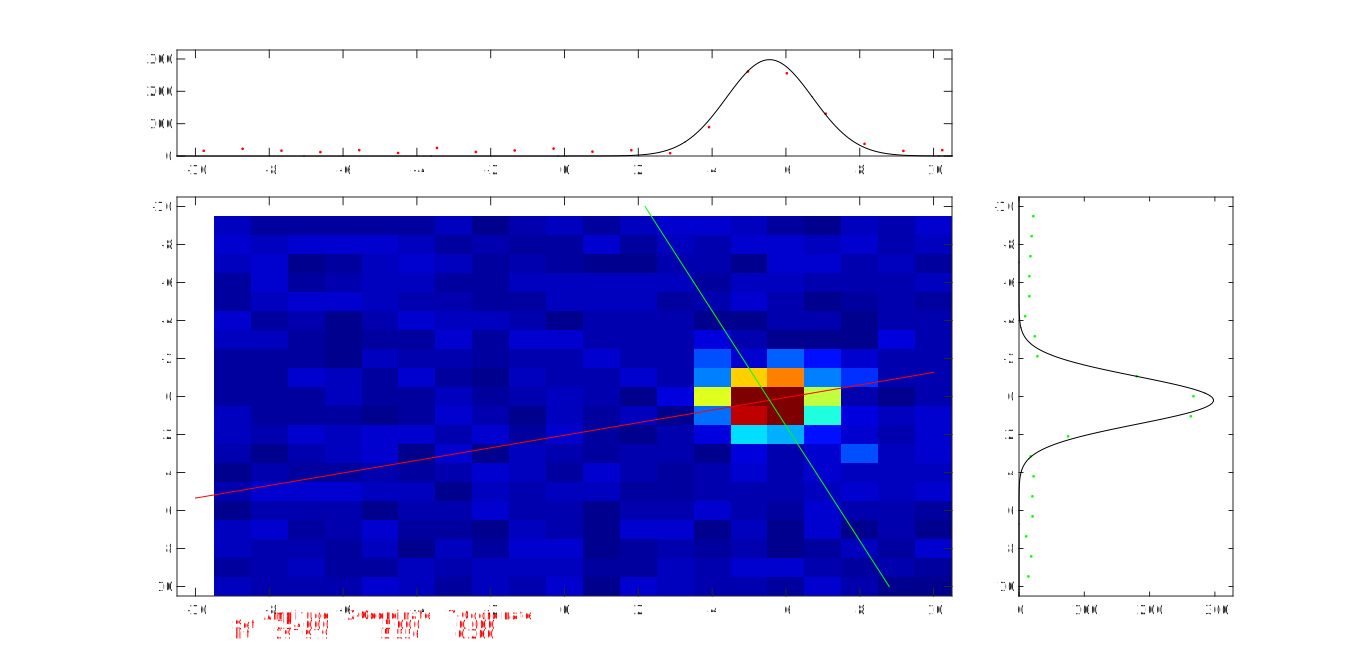
\includegraphics[width=.5\textwidth]{result1}
\caption{Final image generated by applying localisation algorithm on each of the image and summing them to generated an integrated image. }
\end{figure}

\begin{figure}[h]
\centering
\includegraphics[width=.5\textwidth]{result2}
\caption{Final image generated by applying localisation algorithm on each of the image and summing them to generated an integrated image. }
\end{figure}

\begin{figure}[h]
\centering
\includegraphics[width=.5\textwidth]{result3}
\caption{Final image generated by applying localisation algorithm on each of the image and summing them to generated an integrated image. }
\end{figure}

\begin{figure}[h]
\centering
\includegraphics[width=.5\textwidth]{result4}
\caption{Final image generated by applying localisation algorithm on each of the image and summing them to generated an integrated image. }
\end{figure}

\begin{figure}[h]
\centering

\includegraphics[width=.5\textwidth]{final_result.jpg}
\caption{Final image generated by applying localisation algorithm on each of the image and summing them to generated an integrated image. }
\end{figure}


%\section{Lists}

%\subsection{Example for list (3*itemize)}
%\begin{itemize}
%	\item First item in a list 
%		\begin{itemize}
%		\item First item in a list 
%			\begin{itemize}
%			\item First item in a list 
%			\item Second item in a list 
%			\end{itemize}
%		\item Second item in a list 
%		\end{itemize}
%	\item Second item in a list 
%\end{itemize}

%\subsection{Example for list (enumerate)}
%\begin{enumerate}
%	\item First item in a list 
%	\item Second item in a list 
%	\item Third item in a list
%\end{enumerate}
%%% End document
\end{document}